\documentclass[a4paper, 12pt]{article}
\usepackage{graphicx}
\usepackage{float}
\graphicspath{{Images/}}
\usepackage{hyperref}
\usepackage{booktabs}
\usepackage{array}
\usepackage{textcomp}
\hypersetup{
	colorlinks=true,
	linkcolor=red,
	filecolor=blue,      
	urlcolor=cyan,
}
\title{
	\textbf{D}istributed \textbf{S}oftware \textbf{D}evelopment: \textbf{BusPlanner}\\
	\textbf{Design Description}\\
	\begin{figure}[H]
		\centering
		
\includegraphics[width=13cm, height=13cm]{Bus_logo}
	\end{figure}
	\date{}
}
\begin{document}
	\begin{table}[t]
		\centering
		\begin{tabular}{| m{6cm} | m{6cm} |}
			\hline
			BusPlanner & Version: 1.0\\
			\hline
			Design Description & Date: 2016-11-11\\
			\hline
		\end{tabular}
	\end{table}
	\maketitle 
	\begin{center}
		\textbf{\Large Revision History}
	\end{center}
	\begin{table}[h]
		\centering
		\begin{tabular}{| m{3cm} | m{3cm} | m{3cm} | m{3cm} |}
			\hline
			\textbf{Date} & \textbf{Version} & \textbf{Description} & \textbf{Author}\\
			\hline
			2016-11-11 & 1.0 & Initial draft & Team\\
			\hline
			&&&\\
			\hline
			&&&\\
			\hline
		\end{tabular}
	\end{table}
\newpage
	\tableofcontents
	\section{INTRODUCTION}

\subsection{Purpose of this document}
The purpose of this document is to describe the acceptance test procedures for the BusPlanner project. These tests will be used to verify that the product meets the requirements presented in the Requirements Document.

\subsection{Document organization}
The document is organized as follows:
\begin{itemize}
	\item Section 1, \textit{Introduction}, gives an overview of this document describing its contents, scope etc.
	\item Section 2, \textit{Test Plan}, describes the testing process, items and environment.
	\item Section 3, \textit{Acceptance Tests}, describes the test cases.
\end{itemize}

\subsection{Intended audience}
The intended audience of this document is composed of:
\begin{itemize}
	\item Development team.
	\item Team supervisors:
	\begin{itemize}
		\item Abhilash Thekkilakattil (MDH).
		\item Elisabetta Di Nitto (POLIMI).
	\end{itemize}
	\item Project customer: Aneta Vulgarakis Feljan (Ericsson).
	\item Stakeholders.
	\item Any developer who is interested into improving our project.
\end{itemize}

\subsection{Scope}
This document aims to describe the testing process and its purpose, that is to ensure the application meets all of its requirements	. For this reason it includes the features and testing procedures, criteria for passing tests and the expected results. 

\subsection{Definitions and Acronyms}

\subsubsection{Definitions}
\begin{center}
	\begin{tabular} { | m{3.5cm} | m{9.5cm} | }
		\hline
		\textbf{Keyword} & \textbf{Definitions}\\
		\hline
		User & A person who requests buses.\\
		\hline
		Fleet Manager & They own the buses and they are the resource managers of the company.\\
		\hline
		Bus Driver & The driver of the company's buses.\\
		\hline
		User Request & Request generated by the users that choose the stops where they want to get on and off the bus.\\
		\hline
		Algorithm & A method used to enhance the scheduling process (static and dynamic).\\
		\hline
		Sprint & A repeatable work cycle which is also known as iteration.\\
		\hline
		Project Customer & The customer who requested the software product.\\
		\hline
		Acceptance Test & The process of verifying that a solution works for the user.\\
		\hline
	\end{tabular}
\end{center}
\subsubsection{Acronyms and abbreviations}
\begin{center}
	\begin{tabular} { | m{5cm} | m{8cm} | }
		\hline
		\textbf{Acronym/abbreviation} & \textbf{Definitions}\\
		\hline
		UI & User Interface\\
		\hline
		GUI & Graphical User Interface\\
		\hline
		MDH & Mälardalens Högskola, Västerås, Sweden\\
		\hline
		POLIMI & Politecnico di Milano, Milan, Italy\\
		\hline
		QA & Quality Assurance\\
		\hline
		DSD & Distributed Software Development\\
		\hline
	\end{tabular}
\end{center}
	\section{BACKGROUND AND OBJECTIVES}
\subsection{Overview} 
The purpose of this project is to help the city of Johannesburg with the bus planning process which, as of now, lacks of efficiency and effectiveness. 

For more information: \url{http://www.fer.unizg.hr/_download/repository/Project_Plan\%5B12\%5D.pdf}

\subsection{High level description of the functionalities}
The BusPlanner project is based on an algorithm that simulates user requests around the city of Johannesburg. These requests are identified by the two bus stops where the user wants to get on and off the bus. Based on this information, the algorithm is able to identify which route reaches both the user's starting and end point, and then assign the user to the bus already covering that route or assign a new bus to that route if the one already covering it is full. 

In this way the process efficiency will be improved and the time needed to do a scheduling will be reduced. Also, the users' waiting time will be dropped from hours to minutes. 

In a real world users will interact with the system by sending requests for a bus, related to a specific position. They will also be able to view the buses' location in the city, thanks to the mapping service the system will make use of. 

On the other hand, bus drivers will receive a notification for each user request, along with all the related information. 

Fleet managers are the company's resource managers: they manage buses, drivers and routes and they have access to all the information related to the past rides.
	\section{HIGH LEVEL SYSTEM ARCHITECTURE}
The system\textquotesingle s main components will be:
\begin{itemize}
	\item \textbf{Firebase}, for the storage of all the information related to both the BusPlanner application and the users' requests.
	\item \textbf{BusPlanner application}, through which all kind of users (fleet managers, bus drivers, passengers) will interact with the system and will be able to use it over the WEB.
	\item \textbf{Mapping service}, to keep track of the position of both buses and users.  
	\item \textbf{User simulation}, to simulate users' requests from a certain position.
\end{itemize}
\begin{figure}[H]
	\centering
	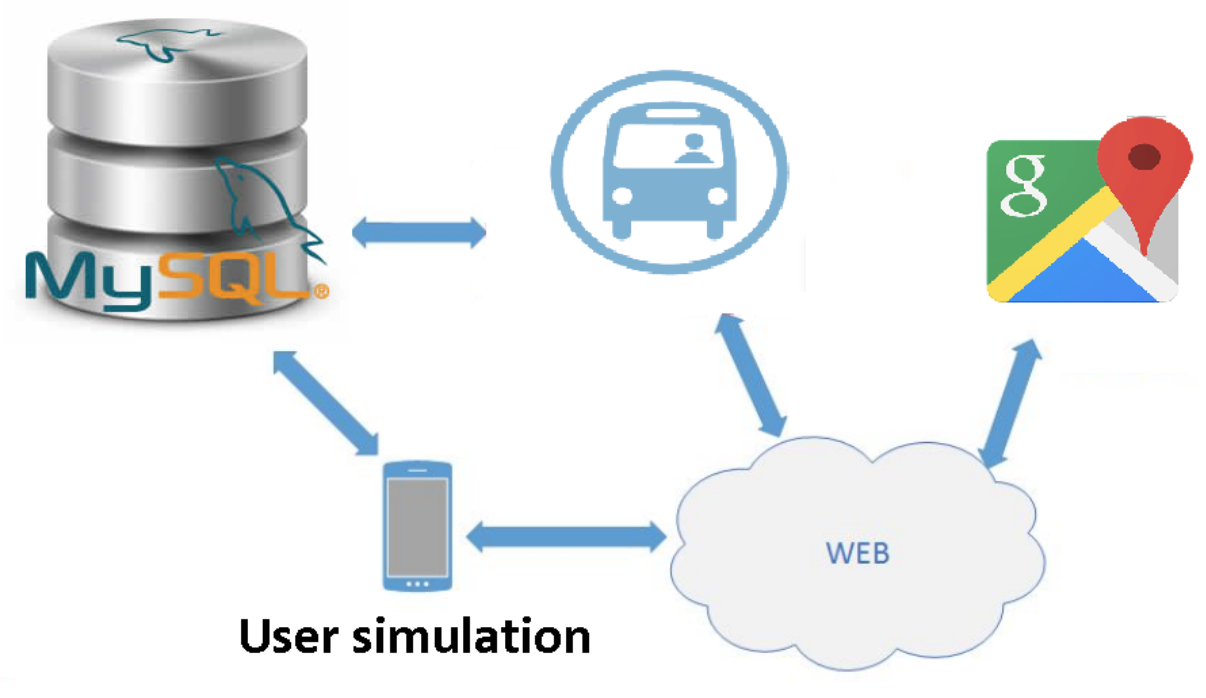
\includegraphics[width=14cm]{System_architecture}
\end{figure}
\subsection{Class diagram}
\begin{figure}[H]
	\centering
	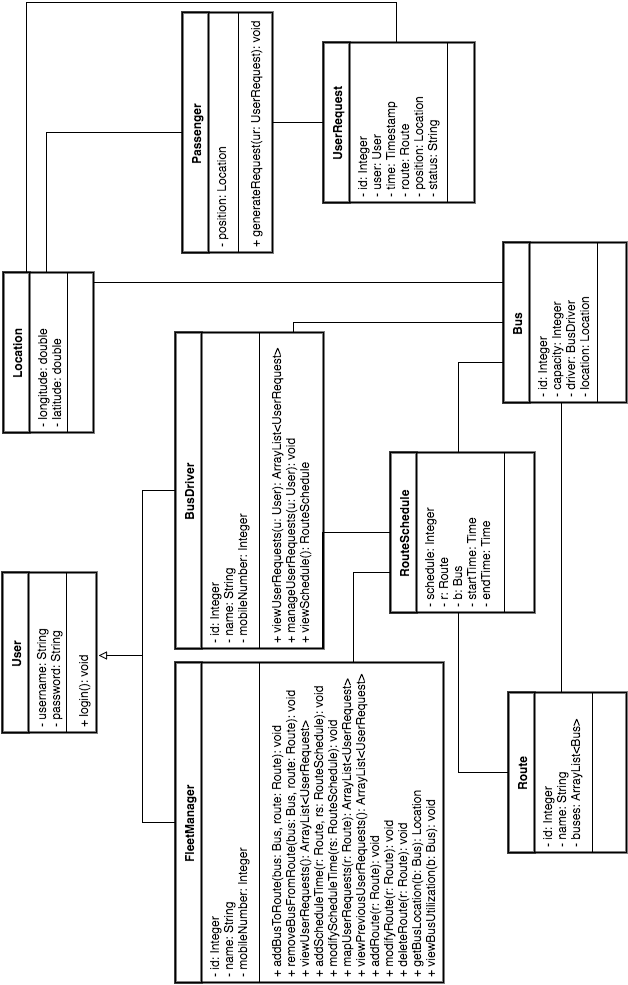
\includegraphics[height=19cm]{ClassDiagram}
\end{figure}
	\section{SOFTWARE ARCHITECTURE}
\subsection{System architecture layers}
The application consists of three layers:
\begin{itemize}
	\item \textbf{Presentation Layer}: contains the components that implement and display the user interface and manage user interaction.
	\item \textbf{Business Logic Layer}: is used as an intermediary for data exchange between the presentation layer and the data access layer. Business entities, or business objects, encapsulate the business logic and data necessary to represent real world elements. The business layer's goal is to minimize the complexity by separating tasks into different areas of concern.  
	\item \textbf{Data Access Layer}: includes methods which can interact with the database. When methods are called, it will connect to the database by using query and will return the corresponding results.  
\end{itemize} 
\begin{figure}[H]
	\centering
	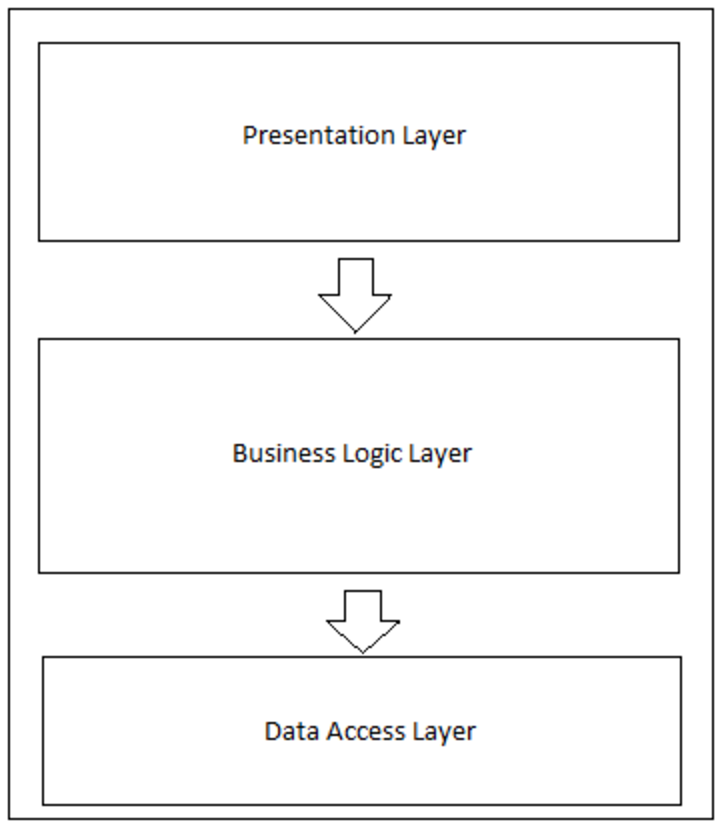
\includegraphics{Three_layered_architecture}
	\caption{Three-layered architecture}
\end{figure}
With a three-layered architecture, improving the modularity of the application will be simple and this can make it easier for developers to extend features in the future. Distinguishing among the different layers allows the development team to program according to the interfaces, thus allowing an easier distribution of the work.  
\subsection{Technologies used}
\begin{itemize}
	\item \textbf{Back-end and database}: PHP will be used to build the back-end of the application and the database used in this application will make use of MySQL.
	\item \textbf{Front-end}: the application will use HTML, CSS and Bootstrap for front-end.
\end{itemize}
\begin{figure}[H]
	\centering
	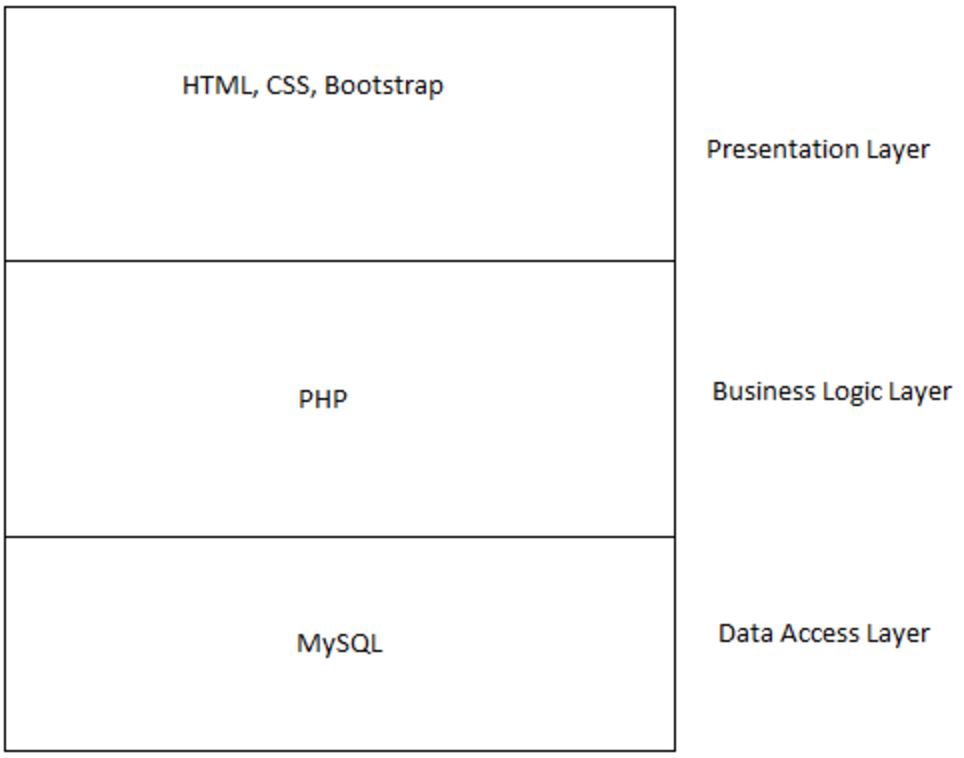
\includegraphics[width=14.5cm]{Technologies}
	\caption{The technologies in the three-layered architecture of the application}
\end{figure}
	\section{GRAPHICAL USER INTERFACE}
The following mockups show a brief overview of the system’s interface. The main goal is to make it easy for the users to interact with the application.
The application’s user are fleet managers and bus drivers; these actors have two different interfaces.
\subsection{Fleet manager's interface}
\begin{itemize}
	\item Fleet manager's homepage:
	\begin{figure}[H]
		\centering
		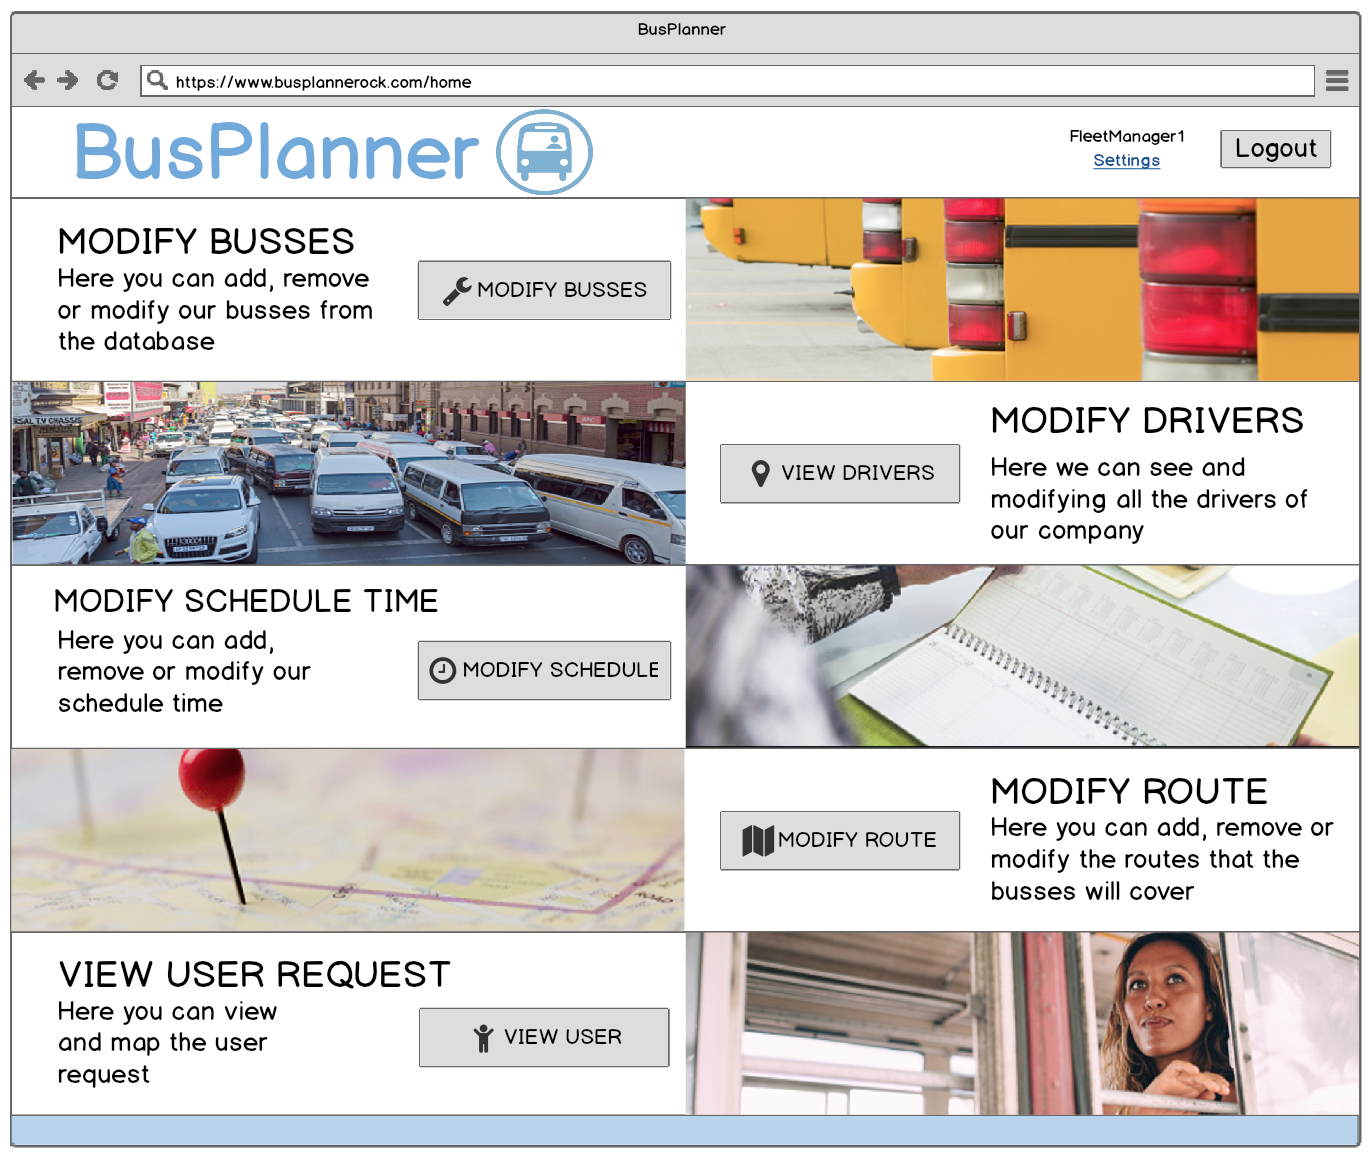
\includegraphics[width=13cm]{HomeFleet}
	\end{figure} 
	\newpage
	\item Adding a bus:
	\begin{figure}[H]
		\centering
		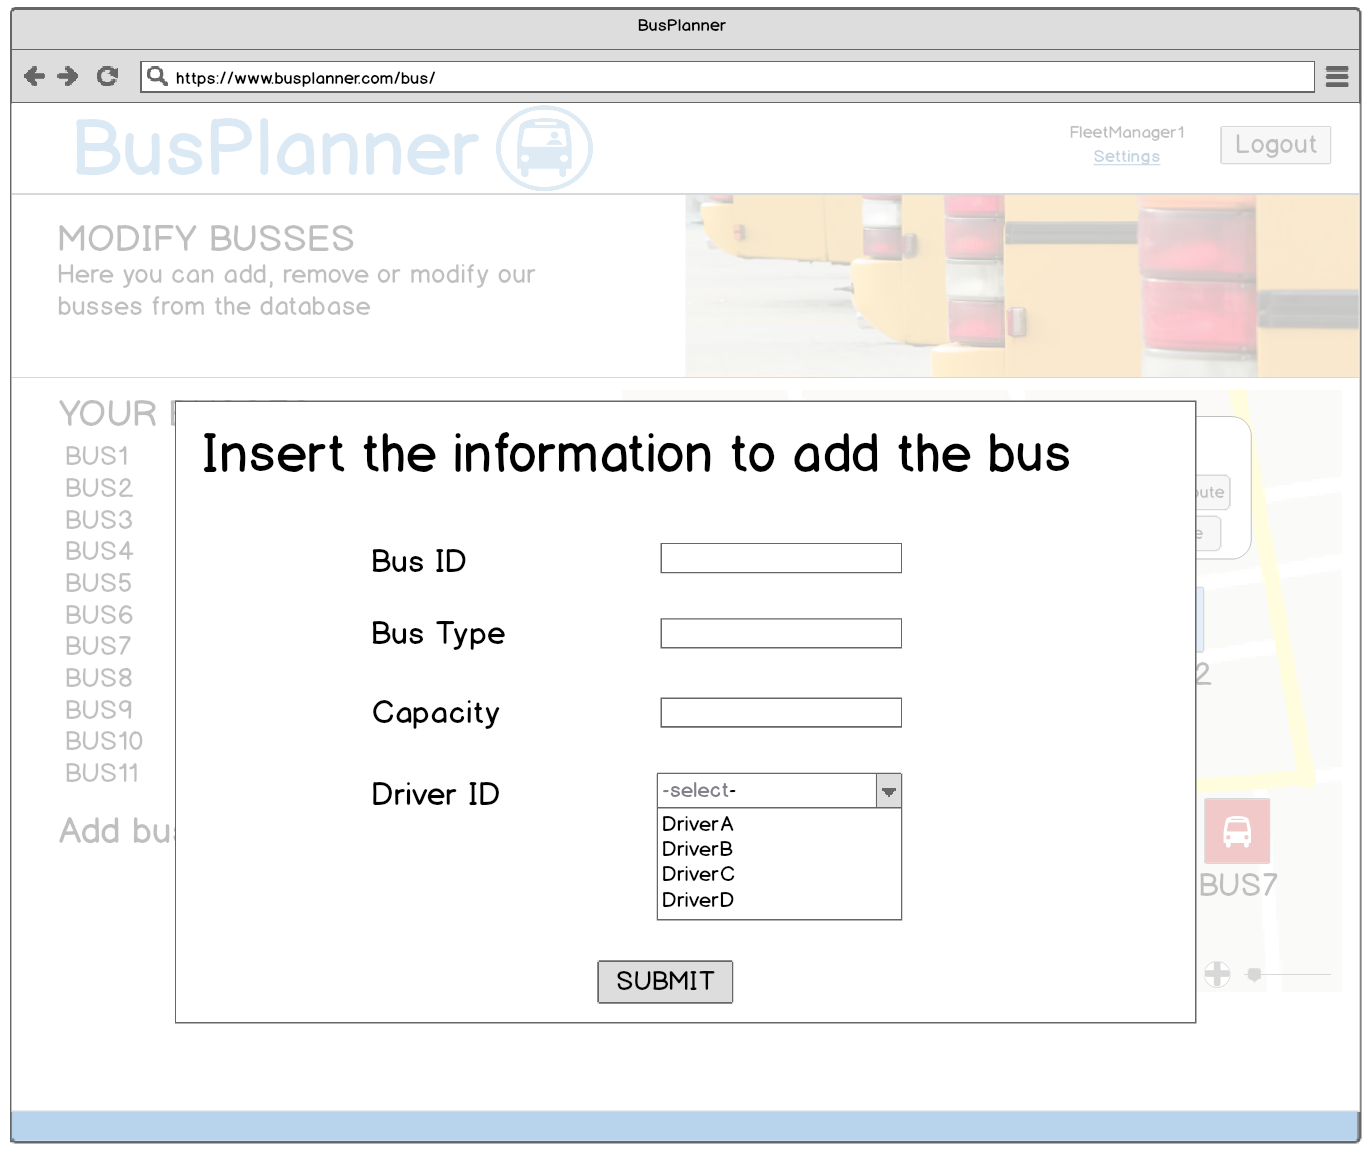
\includegraphics[width=13cm]{AddBus}
	\end{figure}
	\newpage
	\item Buses' list:
	\begin{figure}[H]
		\centering
		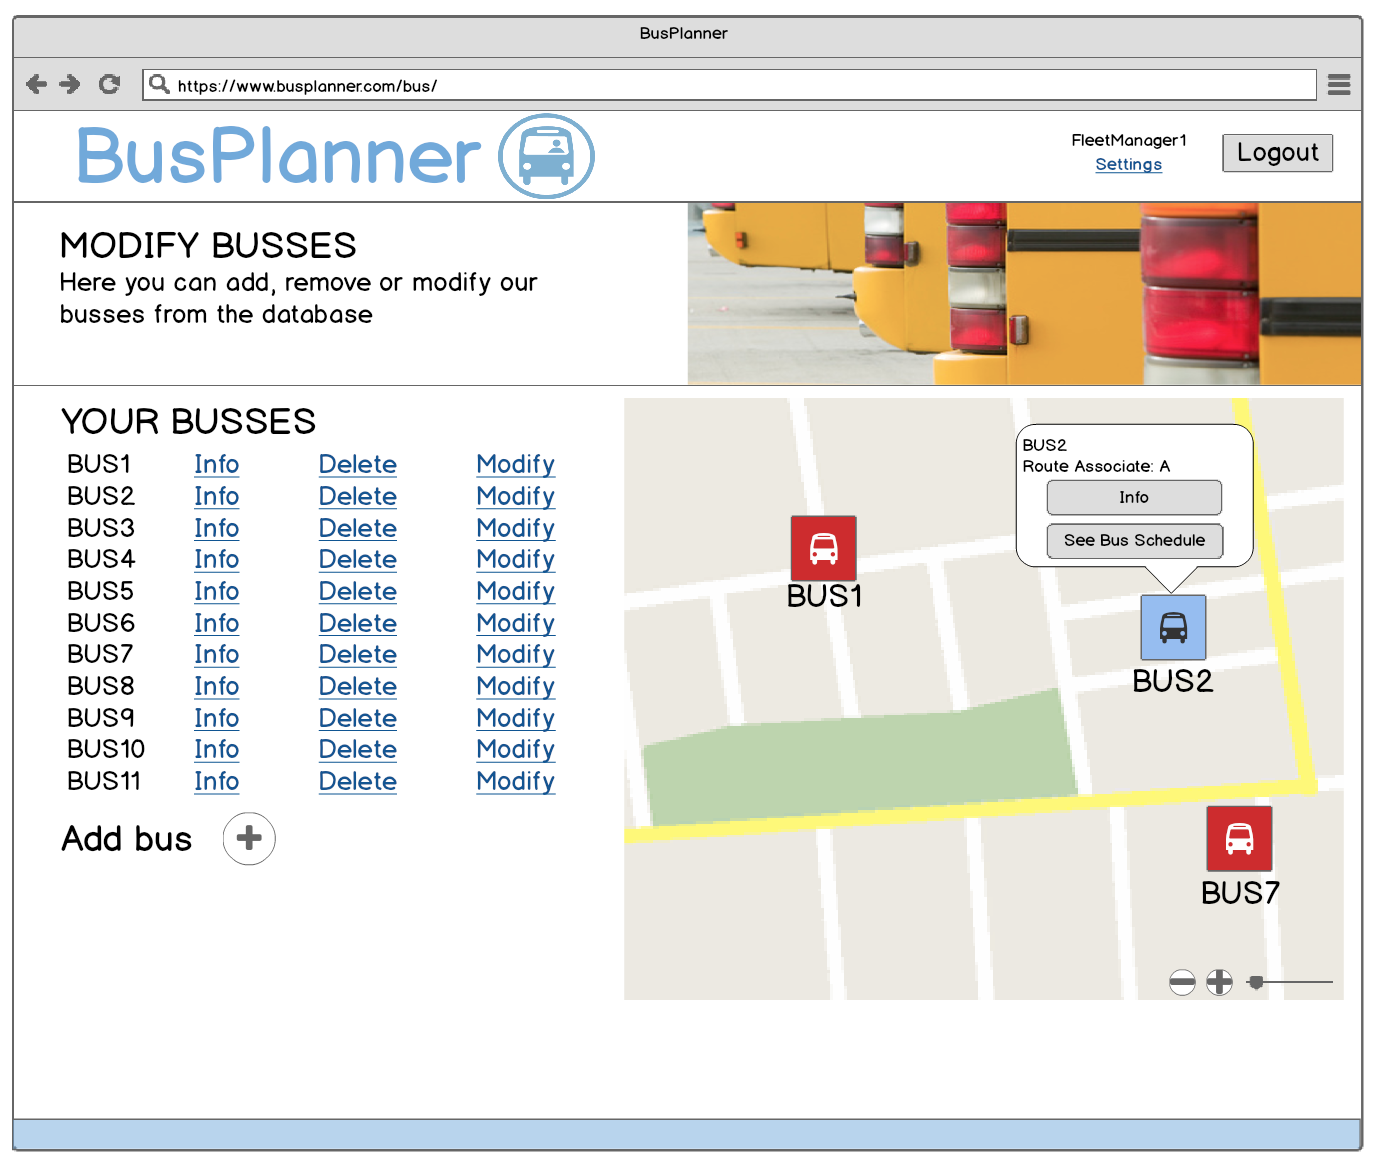
\includegraphics[width=13cm]{BusView}
	\end{figure}
	\newpage
	\item Modify drivers:
	\begin{figure}[H]
		\centering
		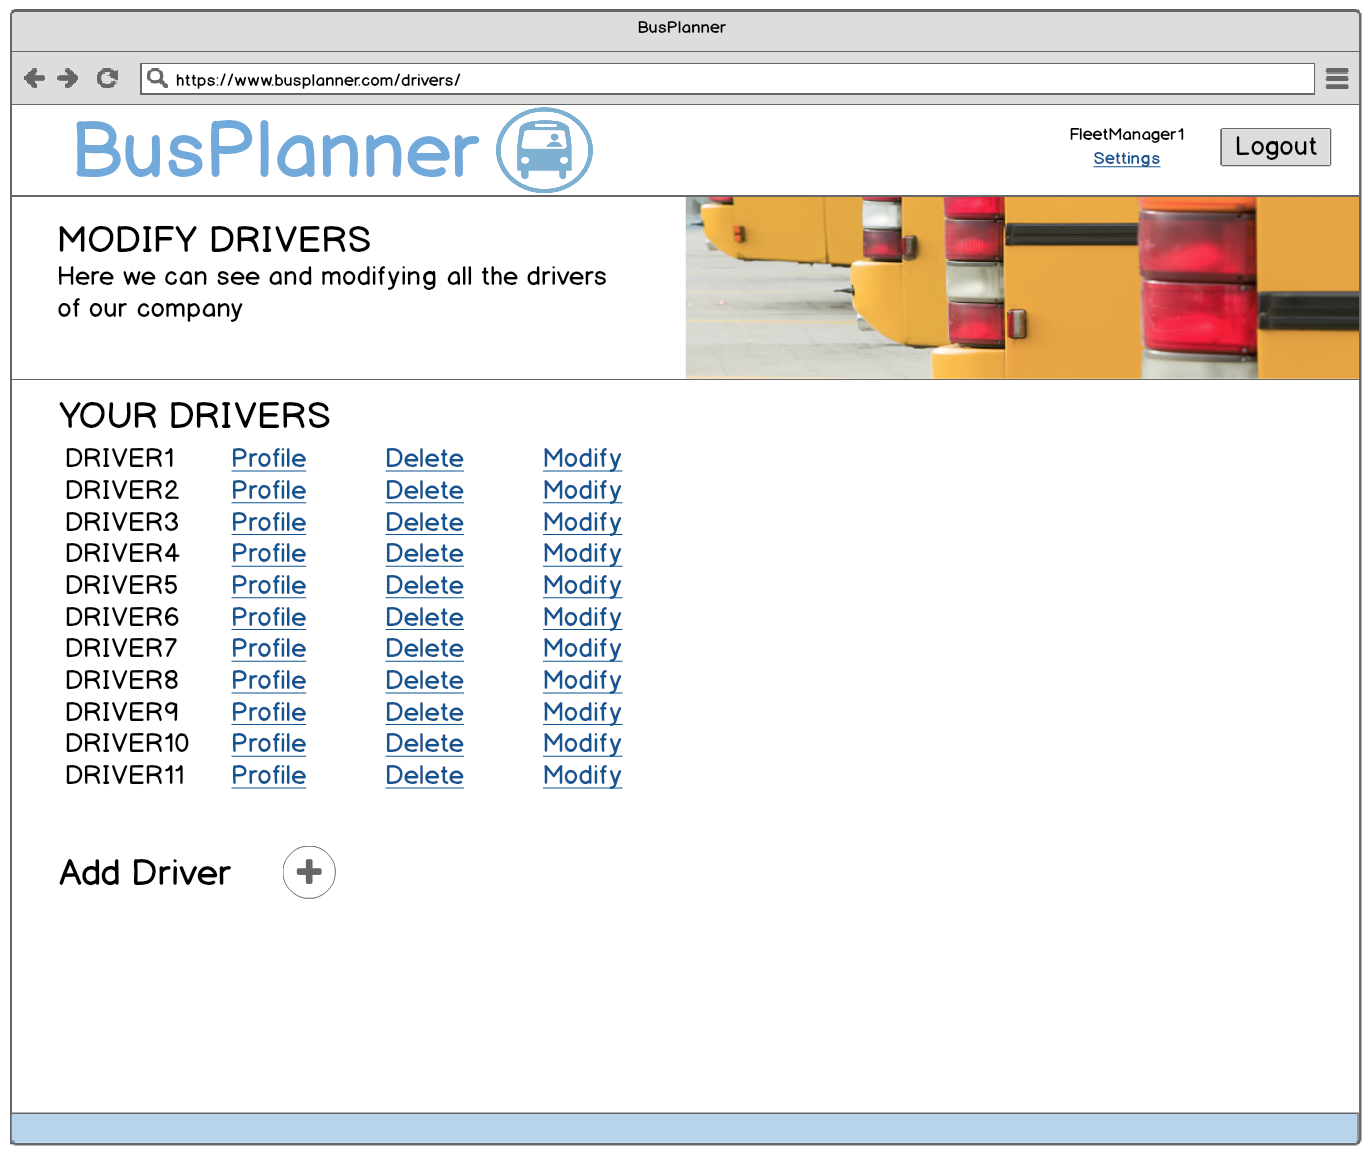
\includegraphics[width=13cm]{DriverView}
	\end{figure}
\end{itemize}
\newpage
\subsection{Bus driver's interface}
\begin{itemize}
	\item Driver's login:
	\begin{figure}[H]
		\centering
		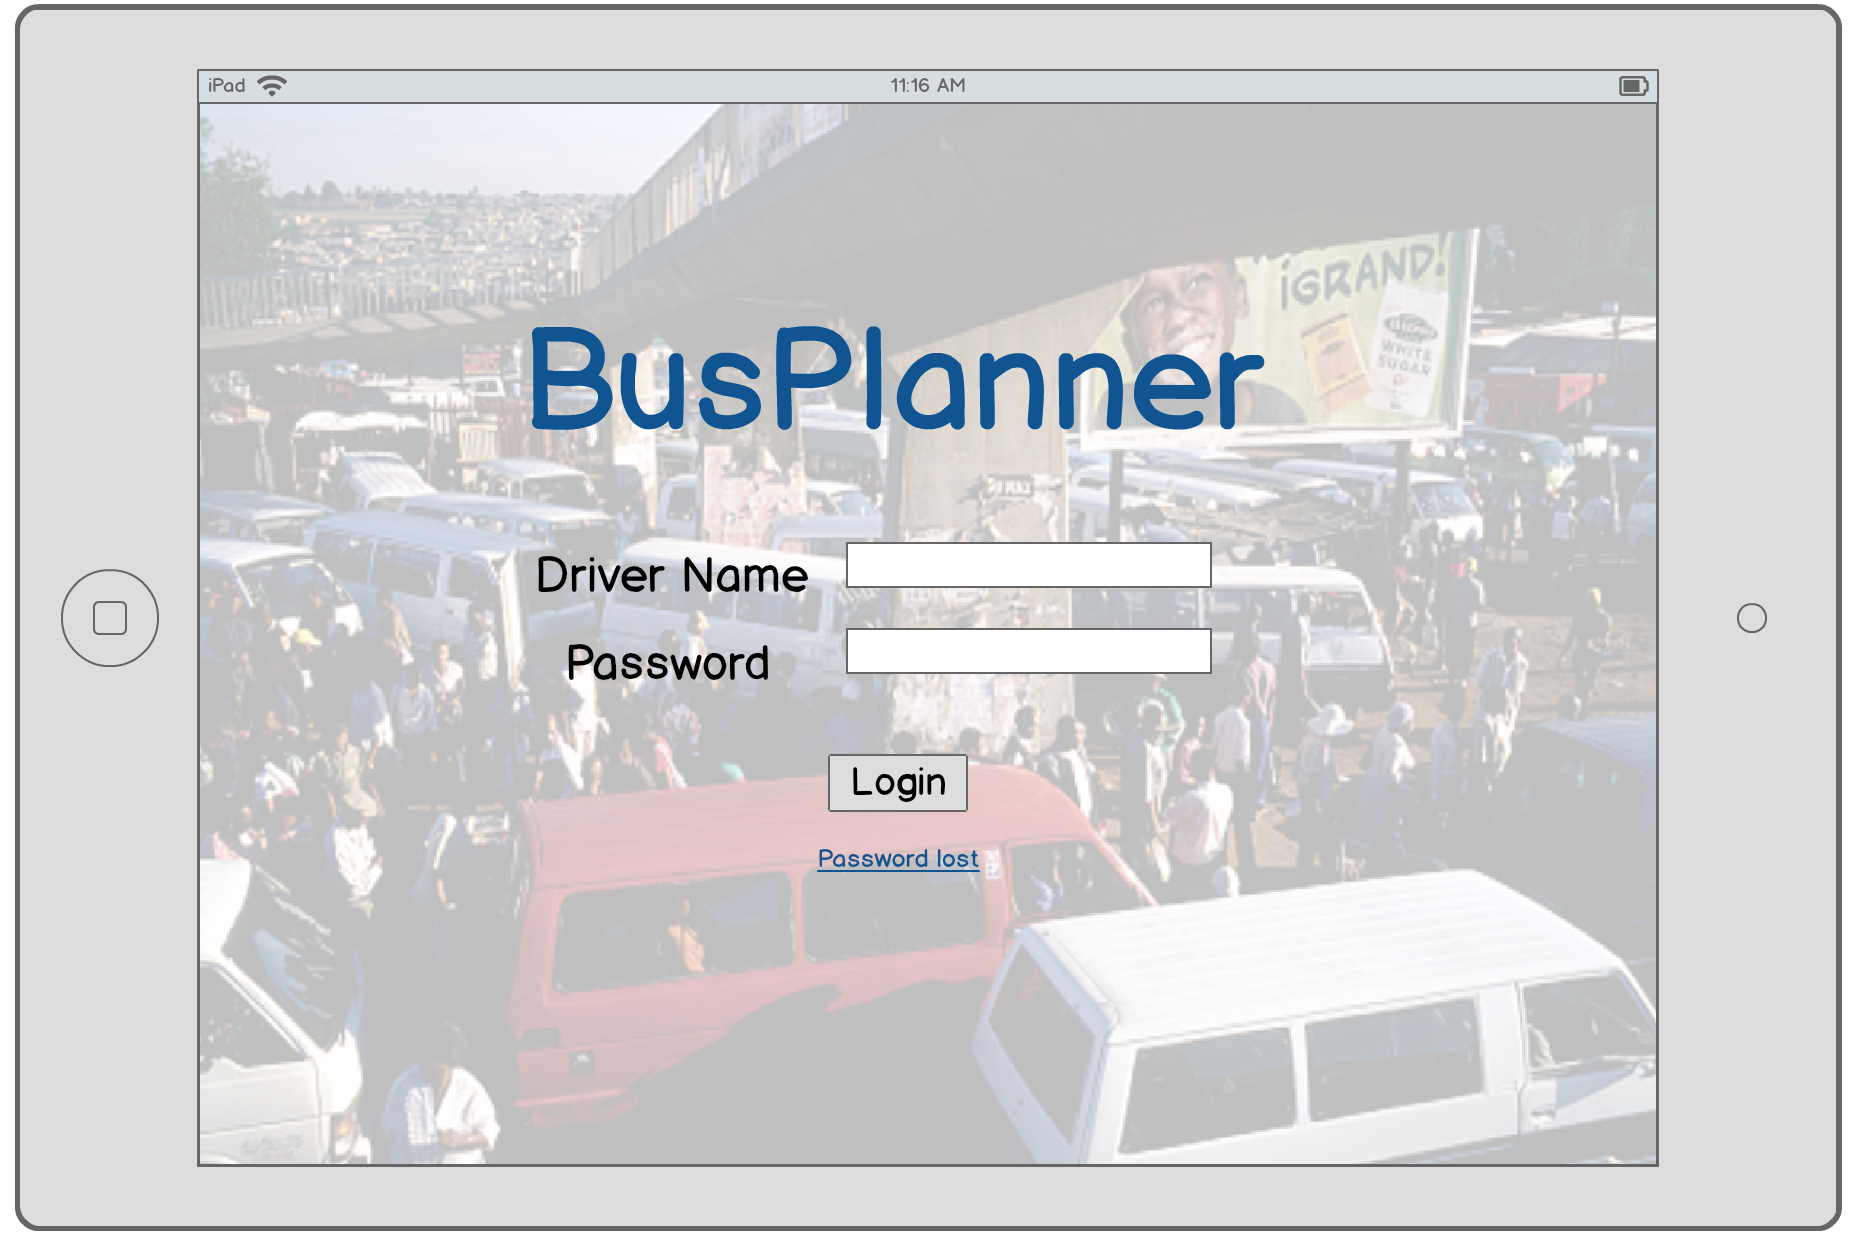
\includegraphics[width=13cm]{LoginDriver}
	\end{figure}
\item Driver's homepage:
\begin{figure}[H]
	\centering
	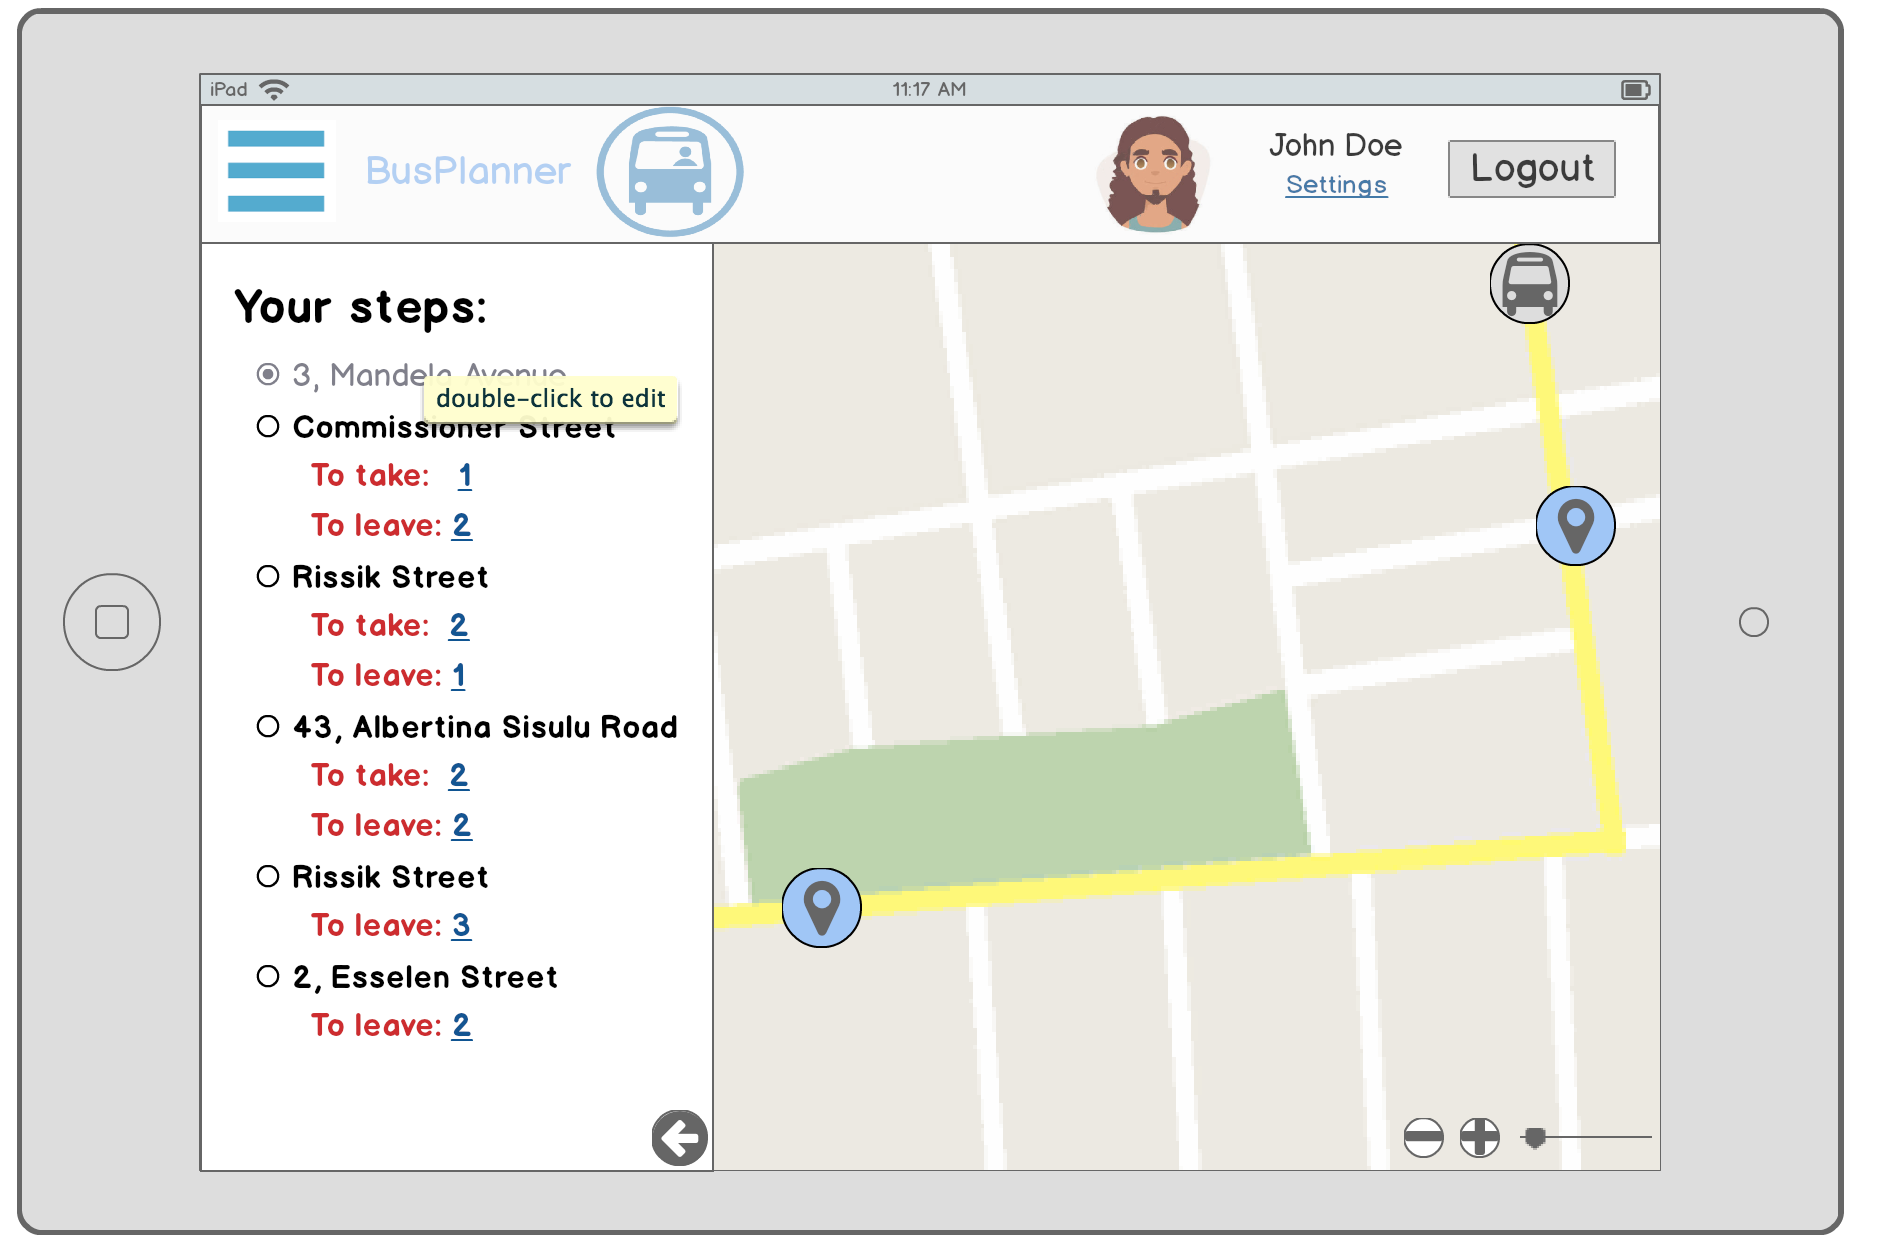
\includegraphics[width=13cm]{HomeDriver}
\end{figure}
\end{itemize}
	\section{DATABASE MODEL}
\setlength{\parindent}{0em}
\textbf{Route}
\begin{table}[H]
	\centering
	\begin{tabular}{| m{4cm} | m{4cm} | m{4cm} |}
		\hline
		Route\_id & integer & PK\\
		\hline
		Route\_name & varchar & \\
		\hline
	\end{tabular}
\end{table}
\textbf{Login}
\begin{table}[H]
	\centering
	\begin{tabular}{| m{4cm} | m{4cm} | m{4cm} |}
		\hline
		Login\_id & varchar & PK\\
		\hline
		User\_name & varchar & \\
		\hline
		Password & varchar & \\
		\hline
		User\_type\_id & integer & \\
		\hline
	\end{tabular}
\end{table}
\textbf{UserType}
\begin{table}[H]
	\centering
	\begin{tabular}{| m{4cm} | m{4cm} | m{4cm} |}
		\hline
		User\_type\_id & integer & PK\\
		\hline
		User\_type & varchar & \\
		\hline
		Login\_id & integer & FK\\
		\hline
	\end{tabular}
\end{table}
\textbf{UserRequest}
\begin{table}[H]
	\centering
	\begin{tabular}{| m{4cm} | m{4cm} | m{4cm} |}
		\hline
		User\_id & integer & PK\\
		\hline
		Timestamp & timestamp & \\
		\hline
		Route\_id & integer & FK\\
		\hline
		Latitude & float & \\
		\hline
		Longitude & float & \\
		\hline
		Status & varchar & \\
		\hline
		Starting\_schedule & integer & \\
		\hline
	\end{tabular}
\end{table}
\textbf{Bus}
\begin{table}[H]
	\centering
	\begin{tabular}{| m{4cm} | m{4cm} | m{4cm} |}
		\hline
		Bus\_id & integer & PK\\
		\hline
		Bus\_type & varchar & \\
		\hline
		Driver\_id & integer & FK\\
		\hline
		Bus\_capacity & integer & \\
		\hline
		Longitude & float & \\
		\hline
		Latitude & float & \\
		\hline
	\end{tabular}
\end{table}
\newpage
\textbf{Driver}
\begin{table}[H]
	\centering
	\begin{tabular}{| m{4cm} | m{4cm} | m{4cm} |}
		\hline
		Driver\_id & integer & PK\\
		\hline
		Driver\_name & varchar & \\
		\hline
		Mobile\_number & varchar & \\
		\hline
	\end{tabular}
\end{table}
\textbf{FleetManager}
\begin{table}[H]
	\centering
	\begin{tabular}{| m{4cm} | m{4cm} | m{4cm} |}
		\hline
		Manager\_id & integer & PK\\
		\hline
		Manager\_name & varchar & \\
		\hline
		Mobile\_number & varchar & \\
		\hline
	\end{tabular}
\end{table}
\textbf{UserSchedule}
\begin{table}[H]
	\centering
	\begin{tabular}{| m{4cm} | m{4cm} | m{4cm} |}
		\hline
		User\_schedule\_id & integer & PK \\
		\hline
		User\_id & integer & FK \\
		\hline
		Driver\_id & integer & FK\\
		\hline
		Bus\_id & integer & FK \\
		\hline
		Route\_id & integer & FK \\
		\hline
		Status & varchar & \\
		\hline
	\end{tabular}
\end{table}
\textbf{RouteSchedule}
\begin{table}[H]
	\centering
	\begin{tabular}{| m{4cm} | m{4cm} | m{4cm} |}
		\hline
		Route\_schedule\_id & integer & PK \\
		\hline
		Start\_time & timestamp & \\
		\hline
		Finish\_time & timestamp & \\
		\hline
		Bus\_id & integer & FK \\
		\hline
		Route\_id & integer & FK \\
		\hline
		Start\_point & varchar & \\
		\hline
		End\_point & varchar & \\
		\hline
		Timestamp\_departure & timestamp & \\
		\hline
		Timestamp\_arrival & timestamp & \\
		\hline
		Number\_onboarding & integer & \\
		\hline
		Number\_debording & integer & \\
		\hline
		Number\_current & integer & \\
		\hline
	\end{tabular}
\end{table}
\end{document}